\section{Sintesi dei materiali}
\diapo{Sintesi di nanoparticelle in micelle inverse}
Il metodo più semplice ed economico per sintetizzare nanoparticelle è la \alert{sintesi in micelle inverse}.\\
\begin{columns}
 \column{0.72\linewidth}
\uncover<2->{
\begin{itemize}
 \item Fonte di selenio: selenio in polvere.
 \item Fonte di cadmio: \alert{ossido di cadmio}\\ (più sicuro del tradizionale dimetilcadmio).
 \item \alert{Passivanti di superficie}: triottilfosfina ossido ed acido tetradecilfosfonico.
\end{itemize}}
\column{0.28\linewidth}
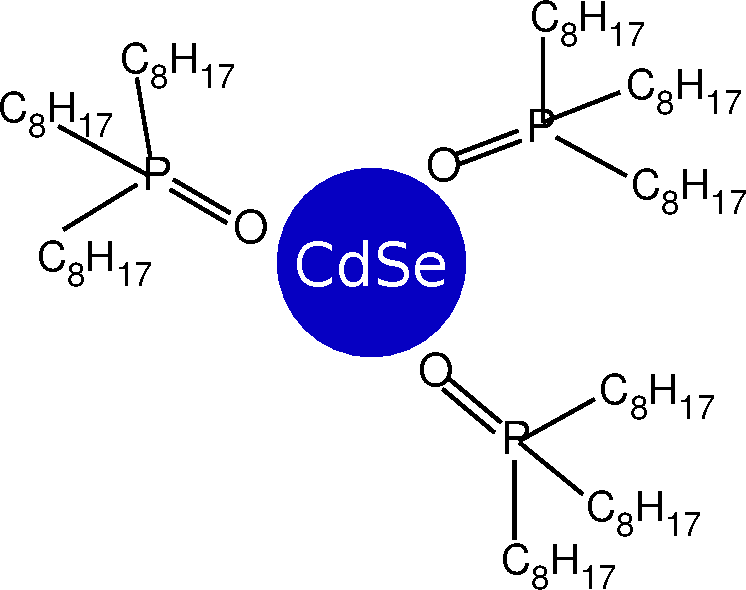
\includegraphics[width=1\textwidth]{Immagini_Tesi/CdSe-TOPO2.pdf}
\end{columns}
\end{frame}

\logo{}


\begin{frame} 
\frametitle{Caratterizzazione UV-vis e TEM}
\begin{figure}
\centering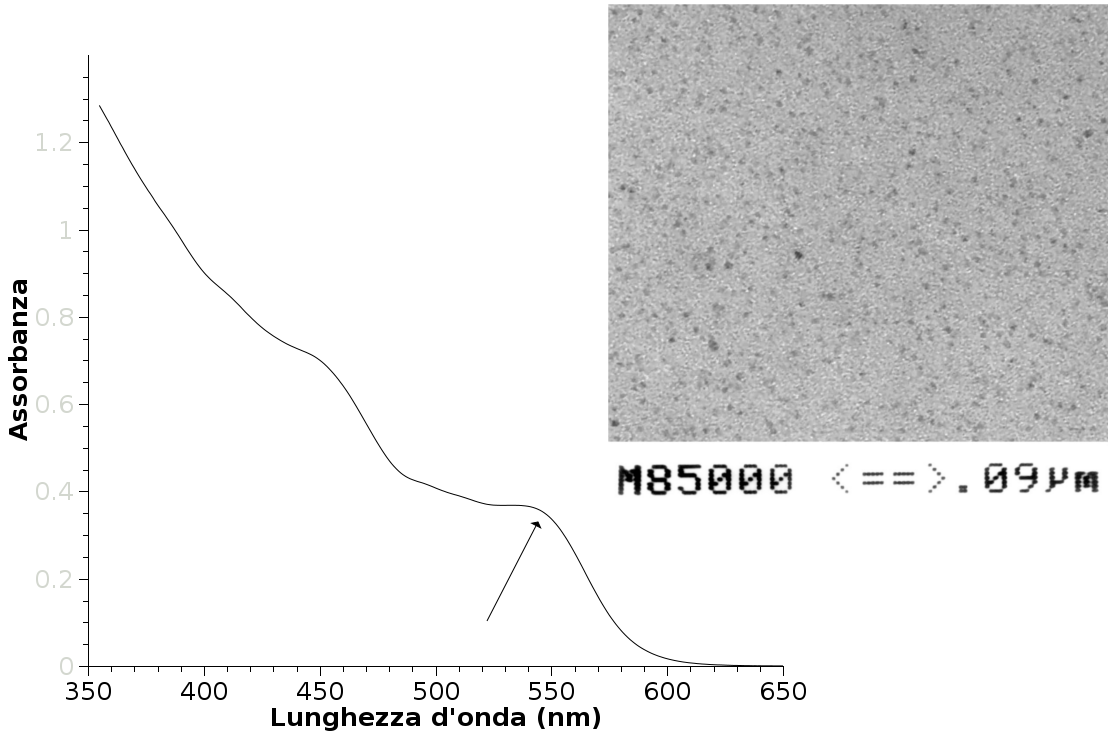
\includegraphics[width=0.9\textwidth]{Immagini_Tesi/caratterizzazione/CdSe-TOPO-UV-TEM.png}
\end{figure}
\end{frame}


%%%%%%%%%%%%%%%%%%%%%%%%%%%%%%%%%%%%%%%%%%%%%%%%%%%%%%%%%%%%%%%%%%%%%%%%%%%%%%%%%%%%%%%%%%%%%%%%%%%%%%%%%%%%%%%%%%%%%%%%%%%%%%%%%%%%


\diapo{Sintesi di poli(3-esiltiofene) regioregolare asimmetrico}

\includegraphics[width=1\textwidth]{Immagini_Tesi/pol-grim-polimerizz3.png}

\end{frame}
{
\setbeamertemplate{navigation symbols}{}
\begin{frame} 
\frametitle{Caratterizzazione $^1$H-NMR}
\vskip -10pt
\begin{figure}
\centering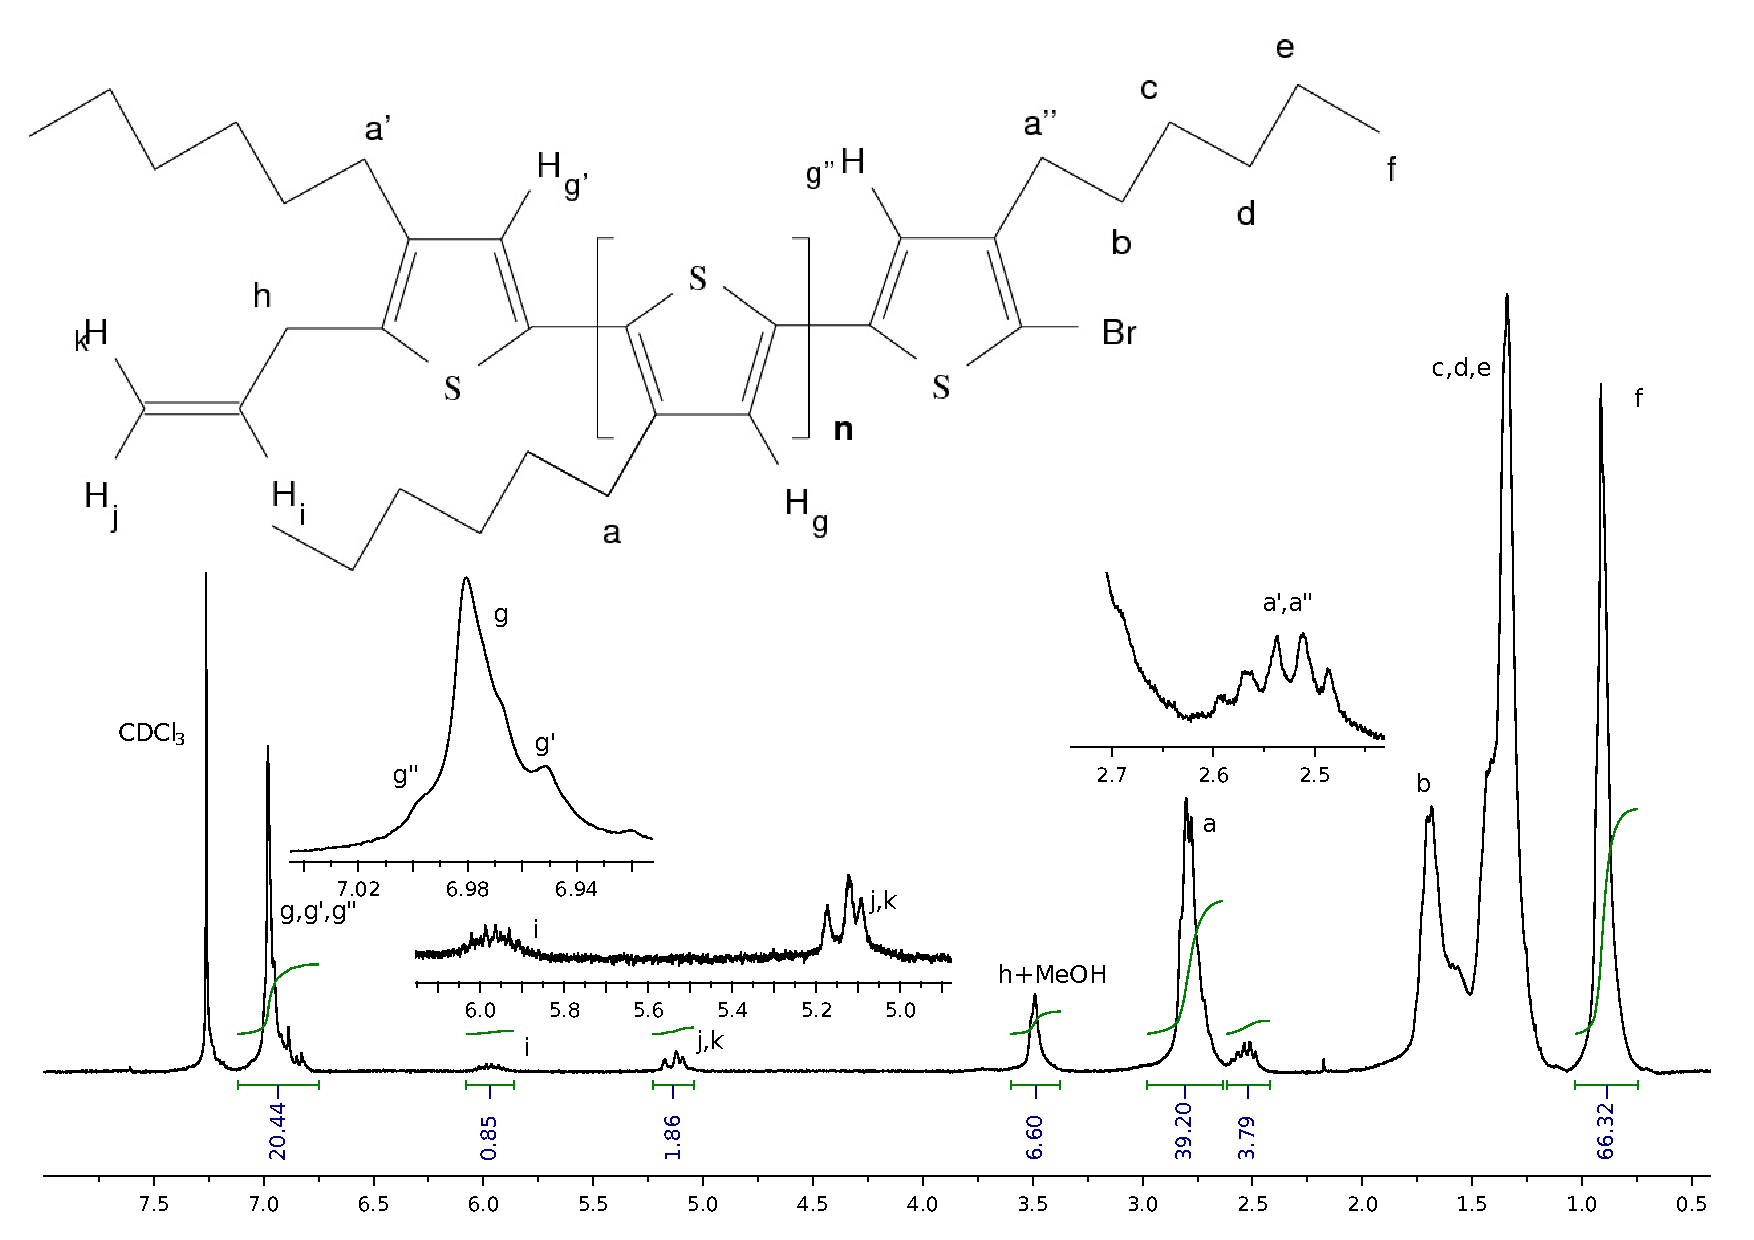
\includegraphics[width=0.98\textwidth]{Immagini_Tesi/caratterizzazione/P3HT-HNMR-3.pdf}
\end{figure}
\end{frame}

}

\logo{\includegraphics[width=0.1\paperwidth]{Immagini_Tesi/logo_unipi/unilogo_small.jpg}}

%%%%%%%%%%%%%%%%%%%%%%%%%%%%%%%%%%%%%%%%%%%%%%%%%%%%%%%%%%%%%%%%%%%%%%%%%%%%%%%%%%%%%%%%%%%%%%%%%%%%%%%%%%%%%%%%%%%%%%%%%%%%%%%%%%%%

\diapo{Attacco del legante ad una terminazione del polimero}
\begin{figure}
\centering{
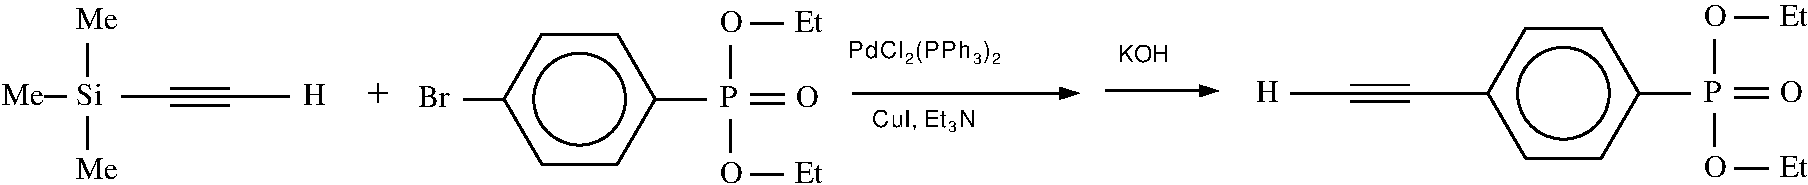
\includegraphics[width=0.8\paperwidth]{Immagini_Tesi/legante2.pdf}}\end{figure}

\begin{figure}
\centering{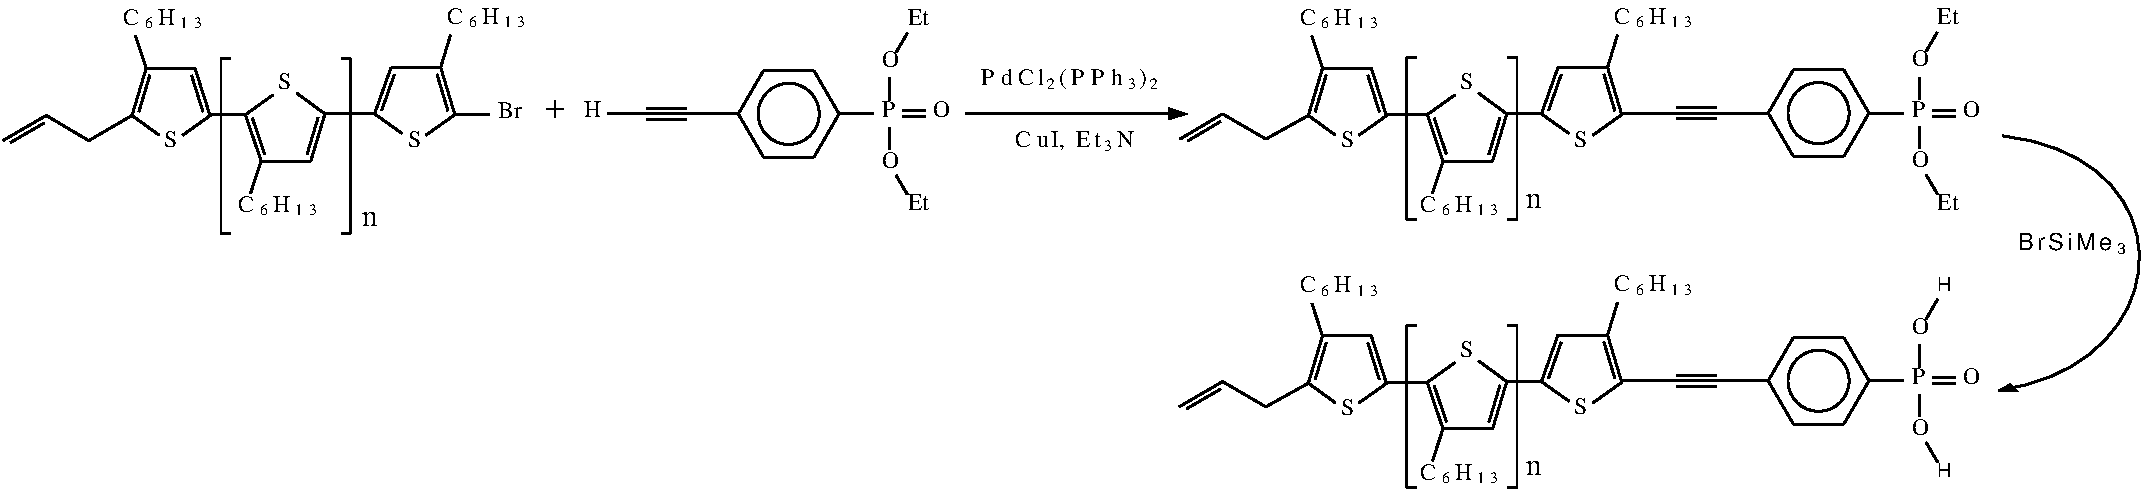
\includegraphics[width=1\textwidth]{Immagini_Tesi/p3ht-legante2.pdf}}\end{figure}
\end{frame}
{
\setbeamertemplate{navigation symbols}{}
\begin{frame} 
\frametitle{Caratterizzazione $^1$H-NMR e $^{31}$P-NMR}
\begin{figure}
\centering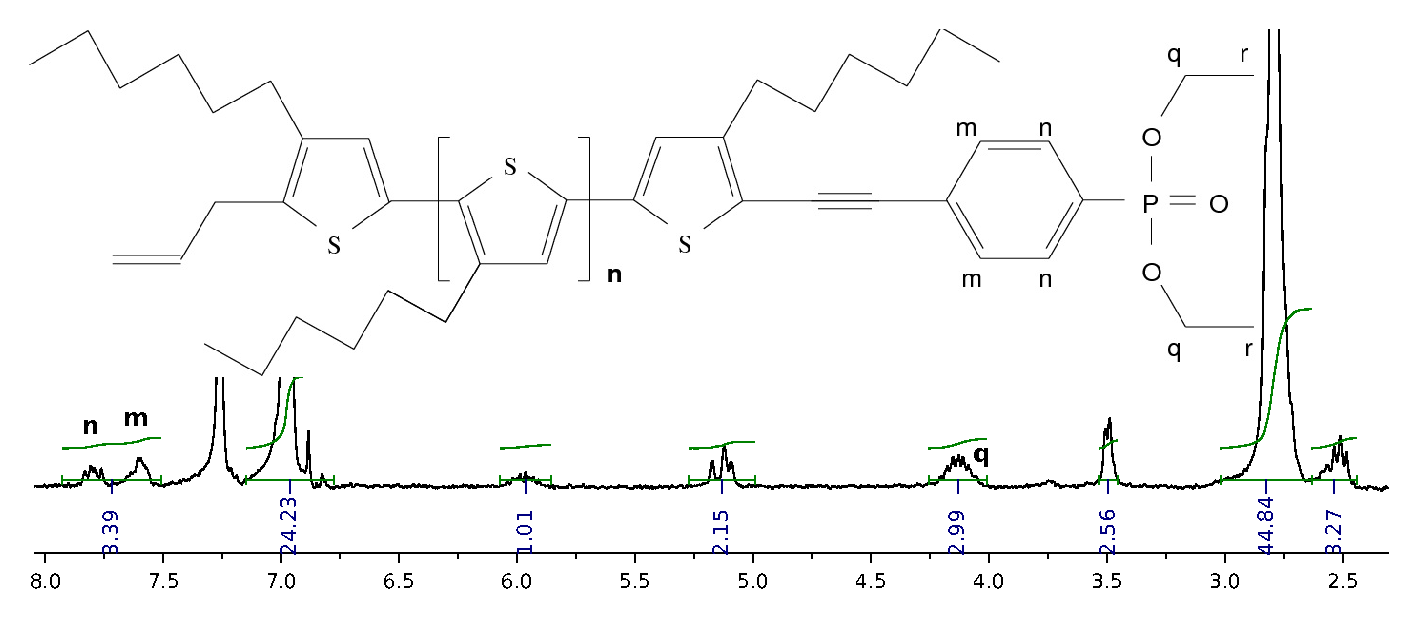
\includegraphics[width=0.85\textwidth]{Immagini_Tesi/caratterizzazione/P3HT-leg-HNMR-3.pdf}\\
\pause
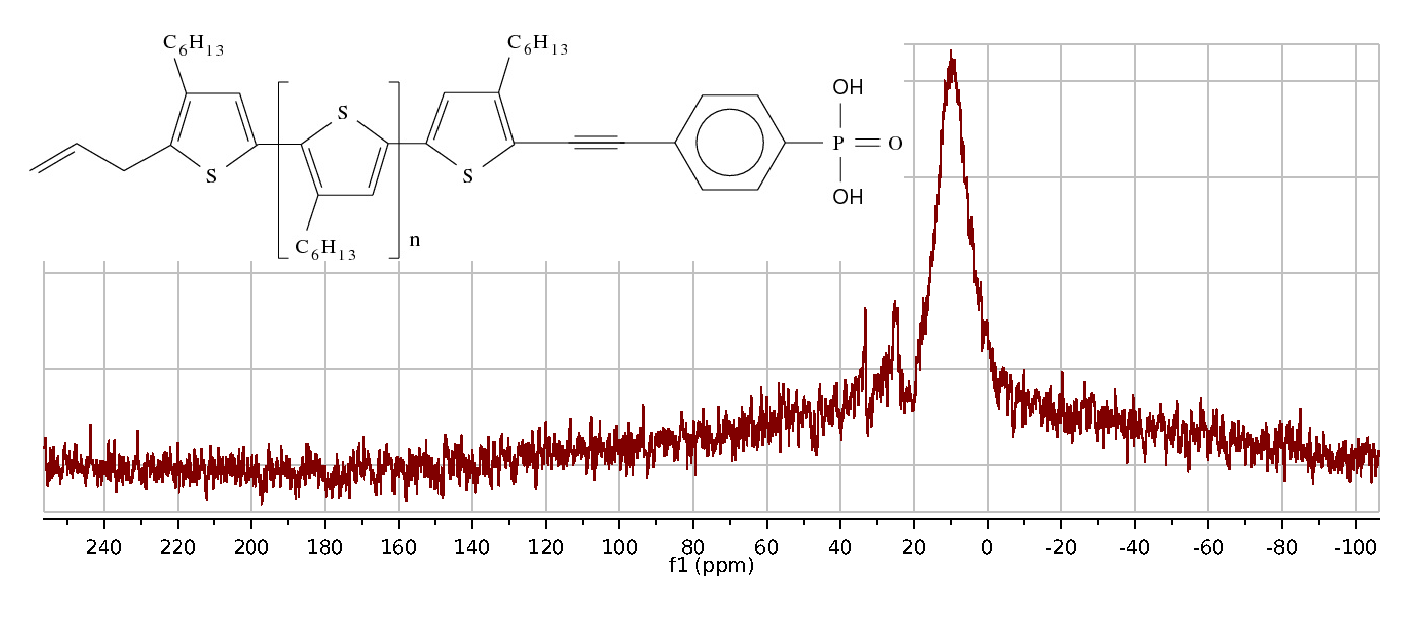
\includegraphics[width=0.7\textwidth]{Immagini_Tesi/caratterizzazione/P3HT-leg-PNMR-2.pdf}\end{figure}


\end{frame}
}
%%%%%%%%%%%%%%%%%%%%%%%%%%%%%%%%%%%%%%%%%%%%%%%%%%%%%%%%%%%%%%%%%%%%%%%%%%%%%%%%%%%%%%%%%%%%%%%%%%%%%%%%%%%%%%%%%%%%%%%%%%%%%%%%%%%%

\diapo{Scambio di leganti sulla superficie delle nanoparticelle}
\begin{figure}
	\centering{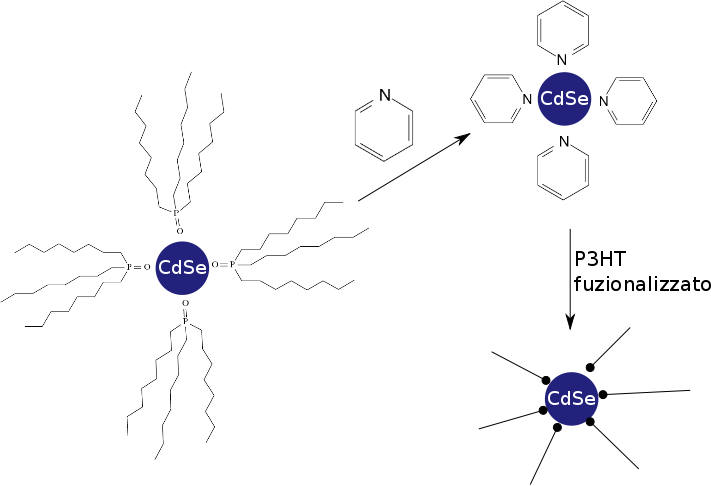
\includegraphics[width=0.8\textwidth]{Immagini_Tesi/scambio-leganti.png}}
      \end{figure}
\end{frame}
\begin{frame} 
\frametitle{Caratterizzazione UV-vis e TEM}
\begin{figure}
\centering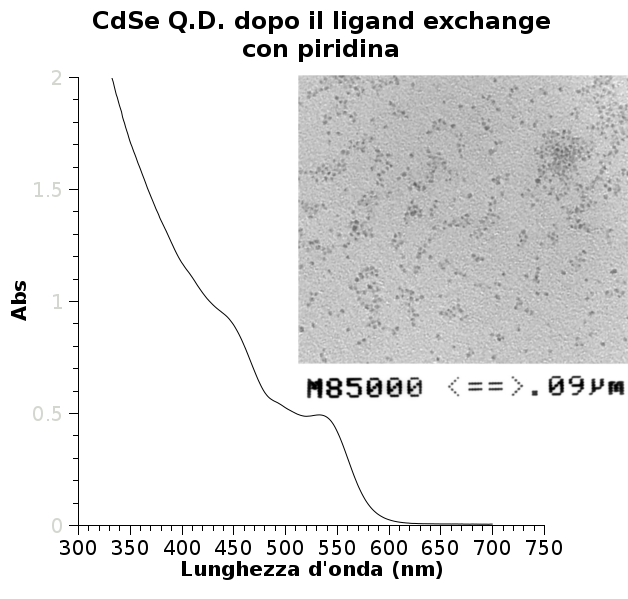
\includegraphics[width=0.5\textwidth]{Immagini_Tesi/caratterizzazione/CdSe-pyr-UV-TEM.png}\pause
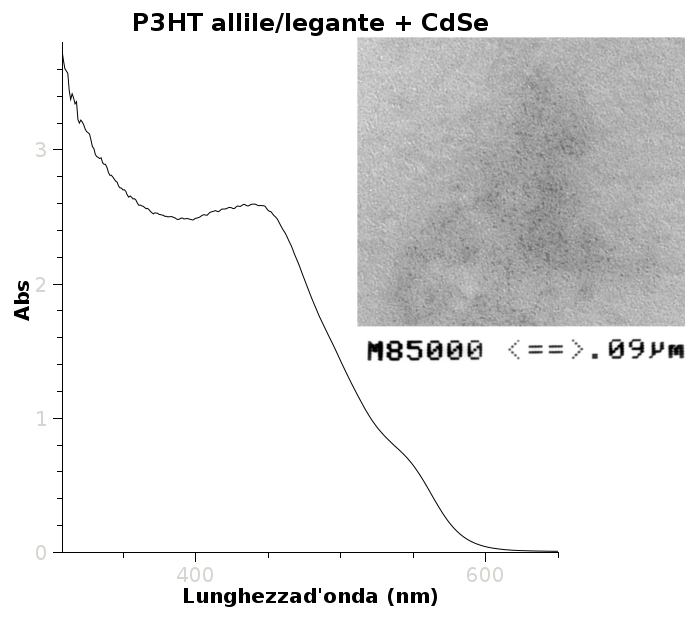
\includegraphics[width=0.5\textwidth]{Immagini_Tesi/caratterizzazione/CdSe-P3HT-UV-TEM.png}\end{figure}


\end{frame}



